\documentclass[polish,12pt]{article}
\usepackage[T1]{fontenc}
\usepackage[utf8]{inputenc}
\usepackage{babel}
\usepackage{a4wide}
\usepackage{geometry}
\geometry{verbose,a4paper,tmargin=3cm,bmargin=3cm,lmargin=2.5cm,rmargin=2.5cm}
\usepackage{epsfig}
\usepackage{pslatex}
\usepackage{setspace}

\begin{document}
\thispagestyle{empty}
~
\vspace{8em}
~
\begin{center}
  
\epsfig{file=surealived-logo.eps, width=8cm}
\end{center}
\begin{center}
  \textbf{\Large Module Writing HOW-TO}\\
  \vspace{2em}
  \large
  Zbigniew Kempczyński\\
  Bartosz Ponurkiewicz
\end{center}
\newpage

\tableofcontents
\newpage
\section{Module data flow}
Testing module (a.k.a \textit{tester}) exports functions called by \textbf{surealived}
according to the following scheme:
\begin{center}
  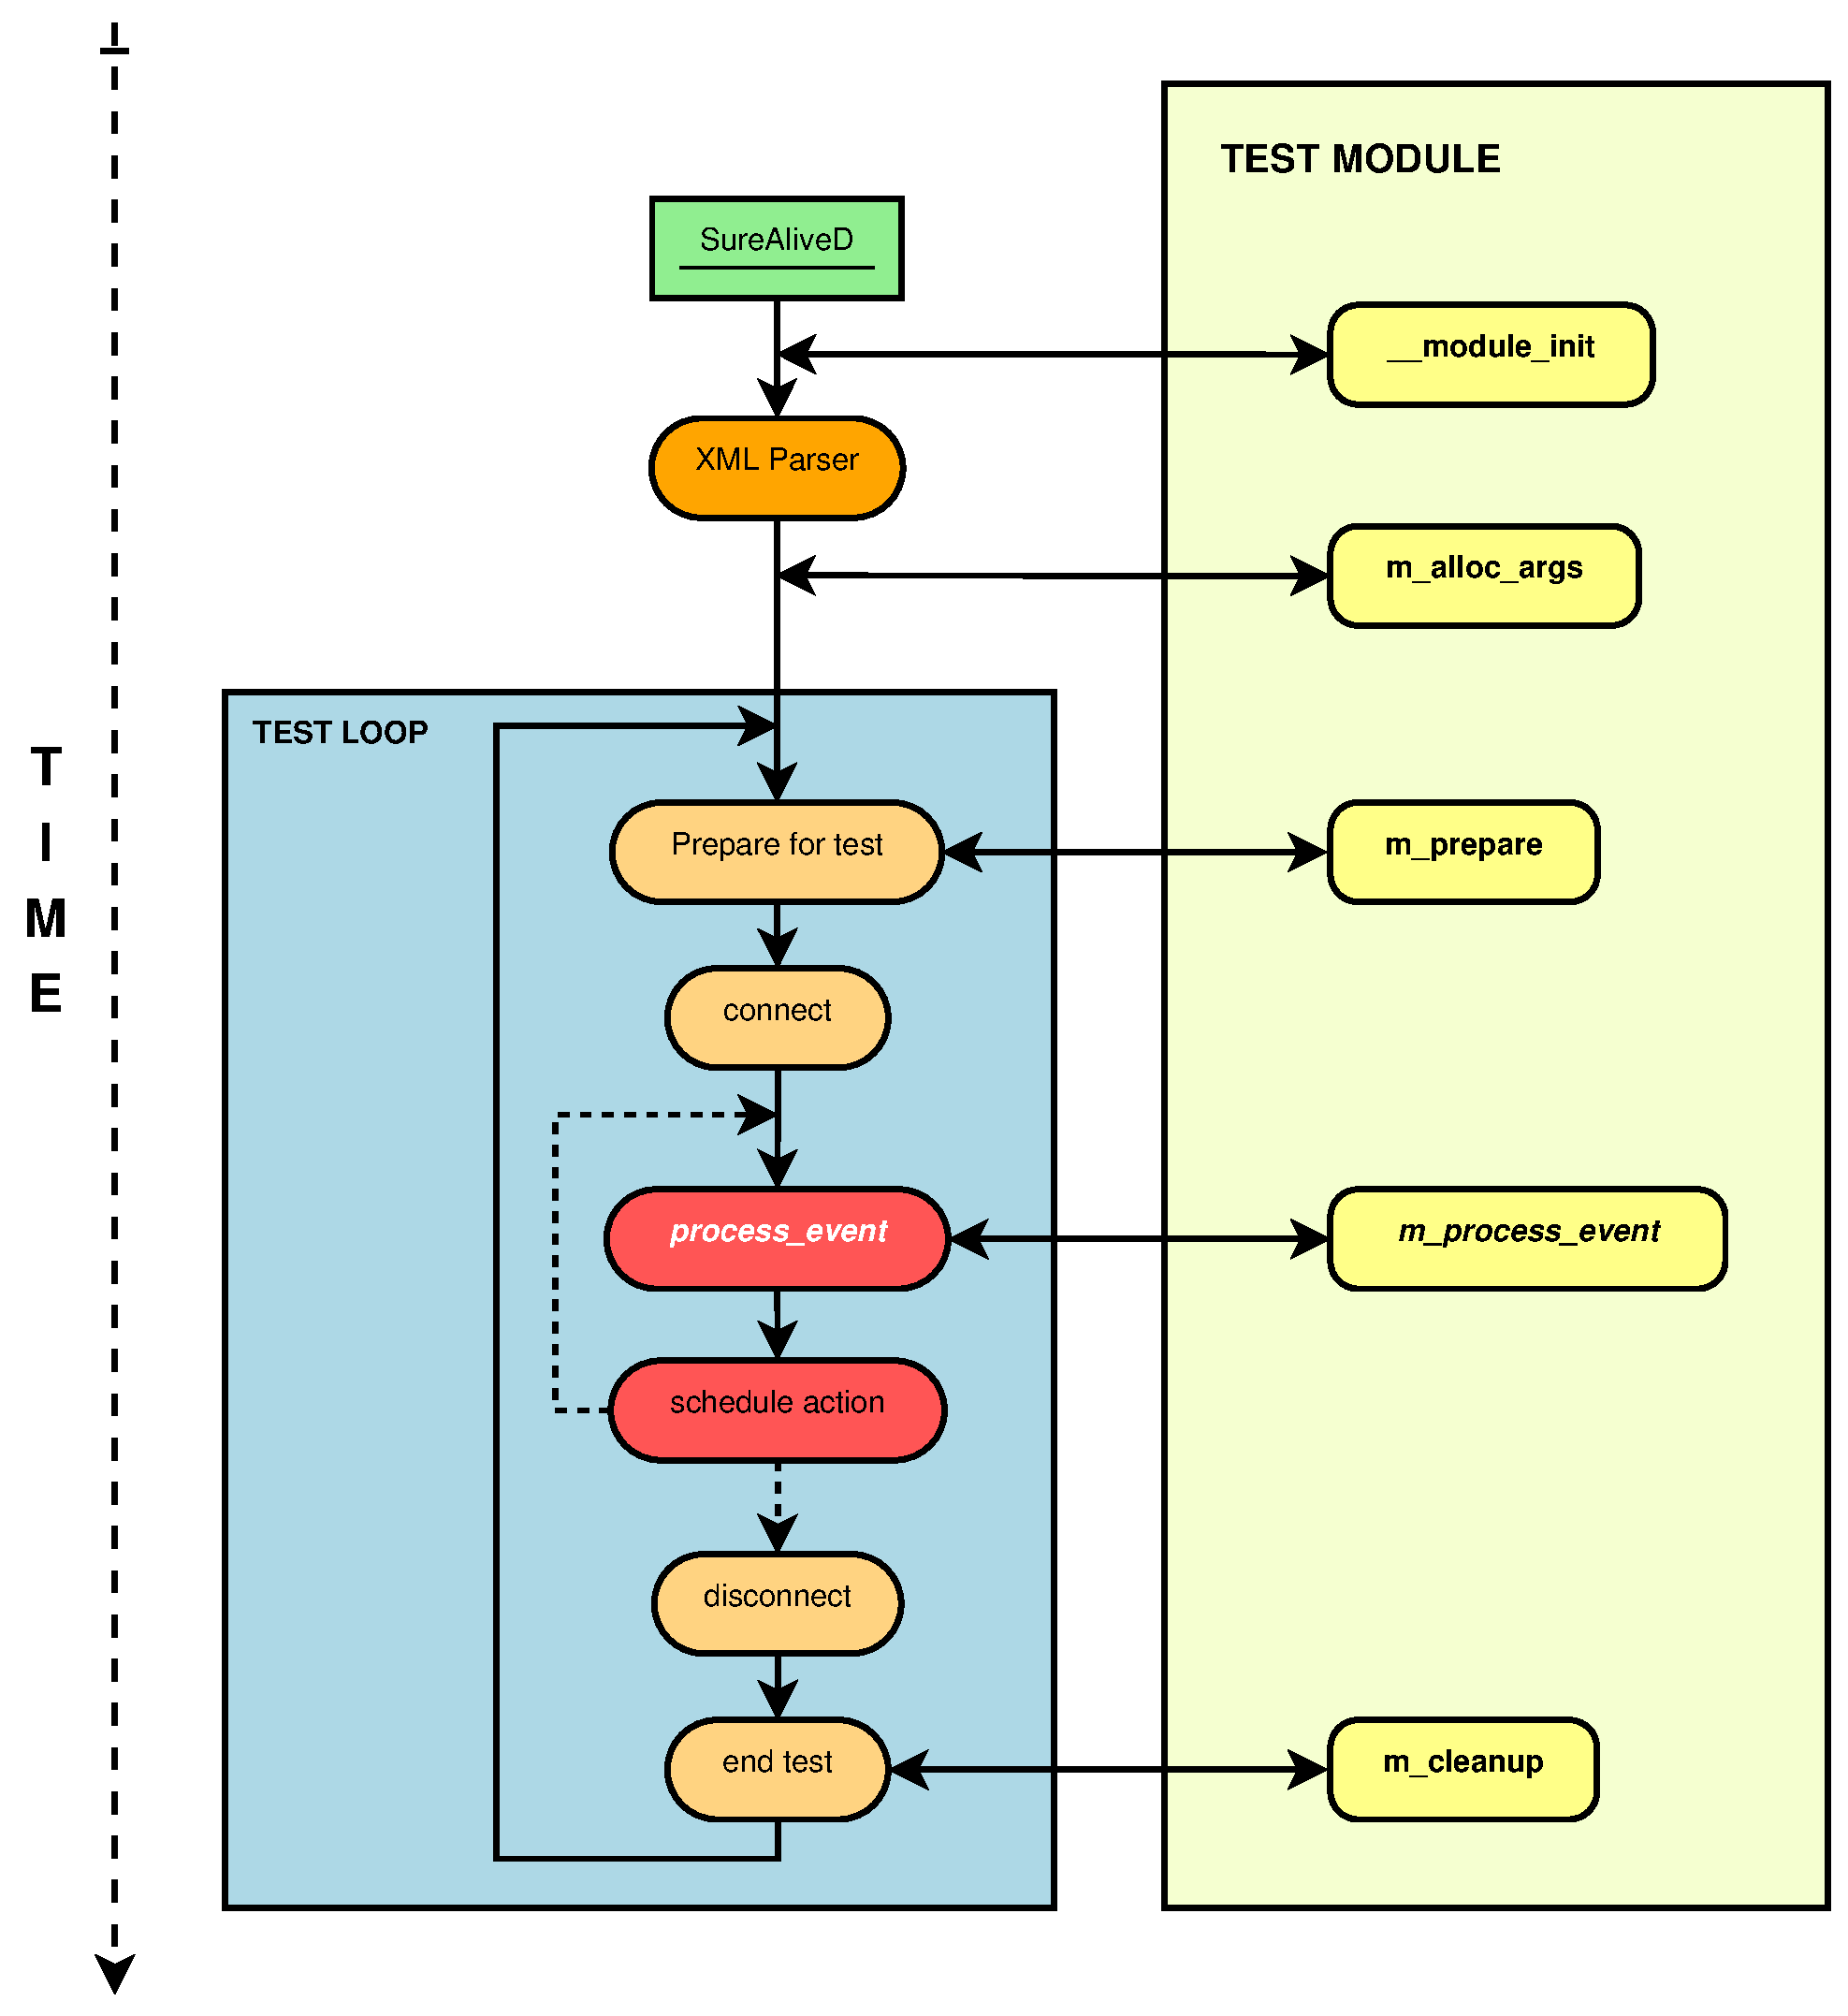
\epsfig{file=module_flow.eps, width=16cm}
\end{center}

\newpage

\subsection{Module information}
Module has to present itself nicely to \textbf{surealived}, to do so it has to declare
and fill \textbf{mod\_operations} structure:
{\small
\begin{verbatim}
typedef struct mod_operations {
    gpointer        (*m_alloc_args)(void);
    void            (*m_free)(CfgReal *); /* free all real's memory */
    void            (*m_prepare)(CfgReal *);
    void            (*m_cleanup)(CfgReal *);
    REQUEST         (*m_process_event)(CfgReal *);
    void            (*m_check)(CfgReal *); /* exec */
    void            (*m_start)(CfgReal *); /* exec */
    gchar           *m_name;
    mod_args        *m_args;
    SDTestProtocol  m_test_protocol;
} mod_operations;
\end{verbatim}
}
Where:
\begin{itemize}
  \item \textbf{m\_alloc\_args} -- pointer to function returning \textit{real's} private structure.
  \item \textbf{m\_free} -- pointer to function free'ing memory when \textit{real} is removed
    from configuration (ie when shutting down server)
  \item \textbf{m\_prepare} -- pointer to function preparing \textit{real} test
  \item \textbf{m\_cleanup} -- pointer to function cleaning up after test
  \item \textbf{m\_process\_event} -- pointer to function handling all events
  \item \textbf{m\_start}/\textbf{m\_check} -- pointers to functions used by \textit{mod\_exec}
  \item \textbf{m\_name} -- module name
  \item \textbf{m\_args} -- pointer to array of \textit{mod\_args} structures
  \item \textbf{m\_test\_protocol} -- type of communication protocol,
    \newline
    possible values are \textbf{SD\_PROTO\_(TCP|UDP|EXEC|NO\_TEST)}
\end{itemize}
\newpage
\subsection{Initialization}
When loading module \textbf{SureAliveD} calls it's init function, which returns
\textit{mod\_args} structure. Module's initializing function \textbf{MUST} be called
\textbf{\_\_init\_module}.\\
Example implementation of this function:
{\small
\begin{verbatim}
static mod_operations mops;   /* Module operations struct */

mod_operations __init_module(void) {
    mops.m_name             = ''http'';
    mops.m_test_protocol    = SD_PROTO_TCP;
    mops.m_args             = m_args;

    mops.m_alloc_args       = module_alloc_args;
    mops.m_prepare          = module_test_prepare;
    mops.m_process_event    = module_process_event;
    mops.m_cleanup          = module_cleanup;
    return mops;
}
\end{verbatim}
}
\subsection{Module's private parameters (per real)}
\textbf{SureAliveD} services configuration is held in XML file.
In that file you may define additional parameters that can control testing modules.
Therefore module must somehow inform \textbf{surealived} which parameters it expects
during configuration. First of all it must create structure that will define possible
variables ie.:
{\small
\begin{verbatim}
typedef struct {
    char        url[BUFSIZ];
    char        host[256];
    char        *request;
    int         req_len;
    bool        naive;
} TestHTTP;
\end{verbatim}
}
\newpage
Besides that module must create NULL-terminated array of \textbf{mod\_args} structures,
which will describe variables used by module. That way \textbf{surealived} will know
how to parse XML configuration.\newline
\underline{mod\_args structure}:
{\small
\begin{verbatim}
typedef struct {
    gchar           *name;        /* attribute name */
    SD_MODARG_TYPE  type;         /* type (STRING/INT/...) */
    guint           param;        /* optional parameter (default value or length) */
    SD_ATTR_TYPE    attr_type;    /* BASIC_ATTR (necessary) or EXTRA_ATTR */
    unsigned long   offset;       /* Use SDOFF makro to define offset */
} mod_args;
\end{verbatim}
}
Where:
\begin{itemize}
  \item \textit{name} -- defines attribute name in XML config
  \item \textit{type} -- argument type, possible types are: \textbf{STRING, PORT, UINT, INT, BOOL}
  \item \textit{param} -- defines maximum length for STRING or default value for other types
  \item \textit{attr\_type} -- defines whether argument is essential (BASIC\_ATTR) or optional (EXTRA\_ATTR)
  \item \textit{offset} -- variable offset from beggining of the structure, it's best to use
    \textbf{SDOFF} makro passing it two arguments -- first is struct name and second is variable name
\end{itemize}
Example:
{\small
\begin{verbatim}
static mod_args m_args[]={
    { "url",     STRING,    BUFSIZ, BASIC_ATTR, SDOFF(TestHTTP, url)     },
    { "host",    STRING,    256,    BASIC_ATTR, SDOFF(TestHTTP, host)    },
    { "naive",   BOOL,      -1,     EXTRA_ATTR, SDOFF(TestHTTP, naive)   },
    { "retcode", INT,       200,    EXTRA_ATTR, SDOFF(TestHTTP, retcode) },
    { NULL, 0,  0,  0,  0 },
};
\end{verbatim}
}
It's not necessary to define all variables from struct, however they will not be set
while parsing (but you can use them as \textit{real's} private data).\\
\underline{That array must be NULL-terminated}.
\newline
Module is responsible for allocating memory for attribute structure, to do so
\textbf{surealived} calls \textit{m\_alloc\_args} declared in \textit{mod\_operations} struct.
\\Example \textit{m\_alloc\_args}:
{\small
\begin{verbatim}
static gpointer module_alloc_args(void) {
    TestHTTP    *ret = g_new0(TestHTTP, 1);
    memset(ret, 0, sizeof(TestHTTP));
    return ret;
}
\end{verbatim}
}
From this moment \textbf{surealived} will handle parsing XML and setting attributes.
Module can be sure that parameters will be set exactly how it is defined in \textit{mod\_args} array.

\subsection{CfgReal struct}
In next steps \textbf{surealived} will pass pointer to CfgReal structure to module's function.
Here are the most important fields of this struct:
\begin{itemize}
  \item \textbf{char *virt->name} -- \textit{virtual} name to which this \textit{real} is plugged
  \item \textbf{char *buf} -- pointer to buffer to/from which \textbf{surealived} will read/write data
  \item \textbf{gboolean test\_state} -- test state TRUE/FALSE
  \item \textbf{char error} -- variable determining whether there was error in transmission
  \item \textbf{u\_int32\_t bytes\_read} -- bytes read in last operation
  \item \textbf{u\_int32\_t intstate} -- \textit{real} internal state (this variable is useful for modules)
  \item \textbf{char name[MAXNAME]} -- \textit{real} name
  \item \textbf{char addrtxt[MAXIPTXT]} -- IP address (human readable)
  \item \textbf{char porttxt[MAXPORTTXT]} -- port (human readable)
  \item \textbf{gpointer moddata} -- pointer to structure allocated by module for specific \textit{real}
\end{itemize}

\subsection{Preparing test}
Before starting the test \textbf{SureAliveD} calls \textit{m\_prepare} function defined
in \textit{module\_operations} struct, it's responsible for setting appropriate values
necessary to run the test (primarily it needs to set \textit{real} state). This
function needs one parameter and it is pointer to \textit{real} config struct -- CfgReal.

\begin{verbatim}
static void m_prepare(CfgReal *real); /* function definition */
\end{verbatim}

\textit{CfgReal} struct contains pointer to \textit{real} private struct defined by module
and allocated by \textit{m\_alloc\_args}, it's name is \textit{moddata}.
Example usage:
\begin{verbatim}
TestHTTP *t = (TestHTTP *)real->moddata;
\end{verbatim}

\newpage

\subsection{Event handling}
\begin{verbatim}
REQUEST m_process_event(CfgReal *real)
\end{verbatim}

Function \textit{m\_process\_event} is called when a new event for \textit{real} is received.
\newline
\newline
Possible error (ie when connection was terminated) is indicated by setting \textit{real->error}
to non-zero value. This function should implement event handling, it also \underline{must} return
it's requests (\textbf{REQUEST} type) to \textbf{surealived}.\\
Possible requests are:
\begin{itemize}
  \item \textbf{WANT\_READ(\textit{n})} -- request to read EXACTLY \textit{n} bytes
  \item \textbf{WANT\_WRITE(\textit{n})} -- request to send EXACTLY \textit{n} bytes
  \item \textbf{WANT\_READ\_AV(\textit{n})} -- request to read AT MOST \textit{n} bytes, but
    module should be notified after first 'read()' from socket.
  \item \textbf{WANT\_EOF} -- request to drain socket, module will be notified when EOF is reached
    \newline all read data is lost
  \item \textbf{WANT\_END} -- request to end test
\end{itemize}
\textit{\textbf{WARNING!} In case of functions requesting reading/writing all operations are
  performed on \textit{buf} pointer from CfgReal struct. Module must ensure that \textit{buf}
  pointer is set correctly and memory to which it points can hold that amount of data.}

\subsection{Cleaning up after test}
\begin{verbatim}
void m_cleanup(CfgReal *real)
\end{verbatim}
If module allocated any data which will not be reused, it should be free'd in this function.
Function \textit{m\_cleanup} is called after the test.

\newpage
\subsection{Example}
In this subsection we will try to describe how \textit{mod\_http.c}, HTTP module works.
{\small
\begin{verbatim}
#include <stdio.h>
#include <glib.h>
#include <common.h>
#include <modloader.h>
#include <sd_defs.h>
#include <xmlparser.h>

#define REQUEST_TEMPLATE "GET %s HTTP/1.0\r\nHost: %s\r\nUser-Agent: SureAliveD\r\n\r\n"
\end{verbatim}
}
These are basic useful include's, but \textit{modloader.h} and \textit{sd\_defs.h} are
necessary for module to work, they contain structures definitions.
REQUEST\_TEMPLATE is (how the name suggests) HTTP request template. It will be filled
with correct host and req.
\begin{verbatim}
typedef struct {
    gchar       url[BUFSIZ];
    gchar       host[256];
    gboolean    naive;
    gchar      *request;
    gint        req_len;
    gchar       ans[64];
    gchar       retcode[4];
} TestHTTP;

enum {
    CONNECTED,
    REQUEST_SENT,
    REQUEST_RECEIVED,
    RECEIVING
} State;
\end{verbatim}

TestHTTP struct contains information used when testing.
State describes \textit{real's} internal state.
\newpage
{\small
\begin{verbatim}
static mod_operations mops;

static mod_args m_args[]={
    { "url",    STRING,     BUFSIZ, BASIC_ATTR, SDOFF(TestHTTP, url)    },
    { "host",   STRING,     256,    BASIC_ATTR, SDOFF(TestHTTP, host)   },
    { "naive",  BOOL,       -1,     EXTRA_ATTR, SDOFF(TestHTTP, naive)  },
    { "retcode", STRING,    4, EXTRA_ATTR, SDOFF(TestHTTP, retcode) },
    { NULL, 0,  0,  0,  0 },
};
\end{verbatim}
}
Here we declare \textit{mod\_operations} struct which will be filled when init
function is called.
\newline
Also \textit{m\_args[]} array is filled with valid \textit{mod\_args} structures.
As you can see module requests two basic attributes -- \textit{url} as STRING of maximal
BUSIZ length and \textit{host} (max 256b). Other attributes are optional -- \textit{naive}
is a boolean value and \textit{retcode} defines expected return code (from webserver).
Last element of ``m\_args'' array MUST be filled with zero's.

\begin{verbatim}
static gpointer module_alloc_args(void) {
    TestHTTP    *ret = g_new0(TestHTTP, 1);
    memset(ret, 0, sizeof(TestHTTP));
    return ret;
}
\end{verbatim}
Function \textit{module\_alloc\_args(void)} allocates and zeroes memory of TestHTTP
size and returns it.
\newline
\newline
\begin{verbatim}
static void module_test_prepare(CfgReal *real) {
    TestHTTP    *t = (TestHTTP *)real->moddata;
    LOGDETAIL("http module test prepare");
    real->intstate = CONNECTED;
    if (!t->retcode[0])
        strncpy(t->retcode, "200", 3);
}
\end{verbatim}
Function preparing \textit{real} to the test primarily sets it's internal state (\textit{real->intstate})
to CONNECTED (\textit{m\_test\_prepare} is called AFTER connection is established), then module
checks if alternative returncode was supplied, if not ``HTTP \textbf{200} OK'' is used.
\newpage
\large \textbf{Test handling}\newline
\normalsize
{\small
\begin{verbatim}
static REQUEST module_process_event(CfgReal *real) {
    TestHTTP    *t = (TestHTTP *)real->moddata;

    if (real->error)
        return WANT_END;

    if (real->intstate == CONNECTED) {
        real->intstate = REQUEST_SENT;     /* set next state */

        real->buf = t->request;
        if (t->request)
            return WANT_WRITE(t->req_len);

        t->request = g_strdup_printf(REQUEST_TEMPLATE, t->url, t->host);

        real->buf  = t->request;
        t->req_len = strlen(t->request); /* and try to remember the length of it */

        LOGDETAIL("MOD_HTTP: requesting to write %d(%d) bytes",
                     t->req_len, REQ_LEN(WANT_WRITE(t->req_len)));
        return WANT_WRITE(t->req_len);
    }
\end{verbatim}
}
First, event handling function checks whether there was any error (connection reset)
if so it ends test immediately returning WANT\_END request.
\newline
If there was no error then module inspects \textit{real} internal state,
if it is just CONNECTED, then it changes it's state to REQUEST\_SENT and
changes buf pointer to \textit{real's} private request buffer. After that
module checks whether request was set for that \textit{real}, if not
then it allocates and sets correct request (using url and host from XML).
And after that it returns request to send data (request).
\newline
{\small
\begin{verbatim}
    else if (real->intstate == REQUEST_SENT) {
        real->buf = t->ans;     /* drop answer to buf */
        memset(real->buf, 0, sizeof(t->ans));
        LOGDETAIL("MOD_HTTP: requesting to read %d(%d) bytes",
                     sizeof(t->ans), REQ_LEN(WANT_READ(sizeof(t->ans))));
        real->intstate = REQUEST_RECEIVED;
        return WANT_READ(sizeof(t->ans));
    }
\end{verbatim}
}
If real is in REQUEST\_SENT state, then module changes operation buffer
to real's private buf holding response and zeroes it.
Then it returns WANT\_READ requesting reading of ``sizeof(t->ans)`` bytes.

\newpage
{\small
\begin{verbatim}
    else if (real->intstate == REQUEST_RECEIVED) {
        if (!strncmp(real->buf+9, t->retcode, 3)) {
            LOGDETAIL("REAL ONLINE [virt:%s,%s]!", real->virt->name, real->name);
            real->test_state = TRUE;
        }
        else
            LOGDETAIL("REAL OFFLINE [virt:%s,%s]!", real->virt->name, real->name);

        if (t->naive)
            return WANT_END;

        real->intstate = EOF;
        return WANT_EOF;        /* notify me when you notice eof */
    }
    else {                      /* for statistics */
        LOGDETAIL("EOF on socket - statistics should be sent!");
    }
\end{verbatim}
}
Last but one possible real state is REQUEST\_RECEIVED,
in that state we need to check ``return code'', if everything is OK then module
sets test state (\textit{real->tes\_state}) to TRUE. \newline
After that module checks if \textit{naive} attribute was set (in XML config), if so
then we need to end test, so module returns -- WANT\_END request.
Otherwise real state is set to EOF and WANT\_EOF request is returned indicating
that module wants to be informed when socket is drained. In that case
last ``else'' will handle it.

\begin{verbatim}
static void module_free(CfgReal *real) {
    TestHTTP    *t = (TestHTTP *)real->moddata;
    if (t->request)
        free(t->request);
    t->request = NULL;
}
\end{verbatim}
Function \textit{module\_free} frees memory allocated by module. This function
is called when \textbf{surealived} wants to remove \textit{real} from \textit{virtual}.

\newpage
{\small
\begin{verbatim}
mod_operations __init_module(void) {
    LOGINFO(" ** Init module: setting mod_operations for tester [http]");

    mops.m_name             = "http";
    mops.m_test_protocol    = SD_PROTO_TCP;
    mops.m_args             = m_args;

    mops.m_alloc_args       = module_alloc_args;
    mops.m_prepare          = module_test_prepare;
    mops.m_process_event    = module_process_event;
    mops.m_cleanup          = module_free;
    return mops;
}
\end{verbatim}
}

Function \textit{\_\_init\_module} initializes mod\_operation structure, sets
module name, communication protocol and structure describing arguments passed
to module. It also sets function pointers to functions handling test.
In the end it returns that structure to \textbf{surealived}.
That function MUST be called \_\_init\_module.

\section{Compilation}
Module needs to be compiled to shared library. It can be done using this command:
\begin{verbatim}
gcc -fPIC -shared -Wl,-soname,mod_NAME.so -o mod_NAME.so mod_NAME.c \
    `pkg-config --libs --cflags glib-2.0` `xml2-config --libs --cflags`
\end{verbatim}
Of course mod\_NAME.so and mod\_NAME.c must be renamed according to
module name. Remember that during compilation all header files should
be accessible.
\end{document}
